\section{Quantum Fourier Transform}
\label{sec:qft}

We now apply the circuit resource model to a core building block of
many quantum algorithms: the quantum Fourier transform (QFT).

The QFT is responsible for most of our examples of an exponential quantum
speedup over classical algorithms. It was introduced in Shor's
original paper on finding prime factors and the discrete logarithm
\cite{Shor1995}, and it can be used to solve
other instances of the more general Hidden Subgroup Problem (HSP)
\cite{Lomont2004} over other finite Abelian groups \cite{Nielsen2000}.
It is now known
how to factor without the QFT,
using just phase estimation \cite{Kitaev2002} \cite{Cleve2000}, which may
be desirable due to the fine $\Lambda(R_k)$ controlled-phase rotations involved.
These are difficult to compile into an efficient, fault-tolerant, universal
gateset since it involves non-Clifford single-qubit rotations $\Lambda(e^{i\theta})$.

\begin{equation}
\label{eqn:rk}
\Lambda(R_k) = \left[ \begin{array}{cccc}
1 & 0 & 0 & 0\\
0 & 1 & 0 & 0\\
0 & 0 & 1 & 0\\
0 & 0 & 0 & e^{i\pi / 2^k}
\end{array}
\right]
\end{equation}

However, the QFT is still of practical importance
in determining the
properties of quantum chemical systems
(such as their ground state energies) \cite{Wang2008} as well as in
many algorithms of the late 90s such as
the transform adder by Draper \cite{Draper2000} and extensions to Grover's
search algorithm \cite{Grover1996} \cite{Brassard1998} \cite{Mosca1999}.
While this gives the QFT somewhat of a vintage feel within the community,
it is still a venerable, useful technique.
Therefore, it makes an ideal candidate for analyzing its depth optimization
over the years, using the techniques
of approximation and unbounded fan-out.

In the rest of this section,
we will show how the QFT has been parallelized and its depth decreased from the
initial quadratic
value \ref{subsec:qft-quad} down to
log-linear \ref{subsec:qft-loglin},
linear \ref{subsec:qft-linear}, and logarithmic depth \ref{subsec:qft-log},
as well as circuit space and its error probability, where
appropriate. 

%%%%%%%%%%%%%%%%%%%%%%%%%%%%%%%%%%%%%%%%%%%%%%%%%%%%%%%%%%%%%%%%%%%%%%%%%%%%%%
\subsection{The Discrete Fourier Transform}

As the name implies, the QFT is inspired by the classical, discrete
Fourier transform (DFT) which relates two sets of complex numbers
$\{x_0, x_1, \ldots, x_{N-1}\}$ and $\{y_0, y_1, \ldots, y_{N-1}\}$,
each in different domains.

\begin{equation}
y_k \equiv \frac{1}{\sqrt{N}} \sum_{j=0}^{N-1} x_j e^{2\pi i j k / N}
\label{eqn:dft}
\end{equation}

This is the idea behind the fast Fourier transform (FFT) \cite{Cooley1965}
used in fast
integer multiplication, fast matrix multiplication \cite{Schoenhage1971},
and many other
important applications \cite{Maslen1997}. The QFT performs a different
operation on quantum states, namely it converts between two bases of
quantum states,
say $\{\ket{j}\}$ and $\{\ket{k}\}$, where usually one of these bases is
the computational basis $\{\ket{0}, \ket{1}, \ldots, \ket{N-1}\}$
and the other we call the \emph{Fourier basis}. The complex amplitudes
$x_j$ of a
particular $\ket{j}$ are related to the amplitudes $y_k$ of all the $\ket{k}$
by the discrete Fourier transform in Equation \ref{eqn:dft}.

\begin{equation}
\ket{j} = \frac{1}{\sqrt{N}} \sum_{k=0}^{N-1} e^{2\pi i j k / N} \ket{k}
\end{equation}

\begin{equation}
\sum_{j=0}^{N-1} x_j \ket{j} \rightarrow \sum_{k=0}^{N-1} y_k \ket{k}
\end{equation}

The relationship between the QFT and the DFT can be thought of as the
difference between computing all the probabilities of a certain distribution
and just sampling from a distribution \cite{Cleve2000}. The latter problem is
often much easier. In both cases, we speak of computing the Fourier transform
with respect to the modulus $N$, the number of basis elements.

The application of the QFT in most quantum algorithms
involve encoding some useful information about each state into its phase,
so that after applying the QFT or its inverse, the correct answer is measured
with high probability.

%%%%%%%%%%
% FIGURE %
%%%%%%%%%%
%\begin{figure}
%\caption{Sound recording in the time and frequency domains}
%\end{figure}

%By analogy, in many quantum algorithms we can encode useful information
%into the phases associated with the probability amplitudes of different
%computational basis states. Our usual goal is to interfere these phases
%both constructively and destructively, to maximize the probability of measuring
%the computational basis state that corresponds to a correct answer to our
%problem. The restriction is that we can only do this using local operations,
%that, by operating on a few neighboring qubits at a time. Through this means,
%we are effectively operating on many computational basis states in parallel,
%due to the way quantum states combine through the tensor product structure.

%[somewhere in the previous section, i unveil my famous spectrum picture
%of quantum states, and demonstrate some examples of highly-entangled
%states and product states]

%%%%%%%%%%%%%%%%%%%%%%%%%%%%%%%%%%%%%%%%%%%%%%%%%%%%%%%%%%%%%%%%%%%%%%%%%%%%%%
\subsection{The Product Representation}

%In one domain, we have information encoded in the bits of the computational
%basis states, but these are just encodings, and you can imagine them
%evolving happily in their own separate alternate universes until one of them
%is selected by random chance by a measurement at the end.
%In the second domain, we have the phases of each computational basis state,
%and the way we can get different computational basis states to interact, or
%to create more or less of them, is through two-qubit entangling gates.
%Actually, now we are on thin ice, and I should think carefully about what I
%want to say here, especially as it relates to universality.

Due to the tensor product structure of multi-qubit quantum states, we can
perform the QFT by performing single-qubit and controlled-phase two-qubit
rotations (the $R_k$ from Equation \ref{eqn:rk}). To do this, imagine that
we have an $n$-qubit computational basis state $\ket{j}$ where
qubit $\ket{j_i}$ has significance $2^i$ in our encoding. We now define the
following single-qubit state with a rotation based on the binary fraction
using bits $j_\ell$ through $j_n$, where $0.j_{\ell} j_{\ell-1} \ldots j_{n} =
\sum_{m=\ell}^n 2^{-m}j_m$.

\begin{equation}
\ket{\phi(\ell)} = \frac{1}{\sqrt{2}}\left( \ket{0} +
e^{2\pi i 0.j_\ell j_{\ell-1} \ldots j_n} \ket{1} \right)
\end{equation}

We can enact each $\ket{\phi(\ell)}$ by using $n-\ell$ rotations
$R_k$ from Equation \ref{eqn:rk} controlled on qubits $\ket{j_\ell}$
through $\ket{j_n}$.

We can then express the QFT on a computational basis state $\ket{j}$ as
the following tensor product of rotated single-qubit states, as proved in
\cite{Nielsen2000}.

\begin{equation}
\ket{j_1, j_2, \ldots, j_n} = \bigotimes_{\ell=1}^{n} \ket{\phi(\ell)}
\end{equation}

%\begin{figure}
%\caption{My famous rotating phase wheel picture}
%end{figure}

We note here that all the QFT circuits we will be discussing in this section
assume the modulus is a power of two, namely $N=2^n$. In reality, we may
approximate arbitrary moduli $m$ with $n'$ qubits where
$n' = \lfloor\log m\rfloor + O(1)$ to within error $\epsilon$, which determines
the circuit size and depth polynomially in $1/\epsilon$
as described in \cite{Cleve2000}.

%%%%%%%%%%%%%%%%%%%%%%%%%%%%%%%%%%%%%%%%%%%%%%%%%%%%%%%%%%%%%%%%%%%%%%%%%%%%%%
\subsection{QFT in $O(n^2)$ Depth}
\label{subsec:qft-quad}

The most well-known circuit for the QFT from Nielsen \& Chuang
\cite{Nielsen2000} applies each of the following gates in sequence, as shown
in Figure \ref{fig:qft-serial}.

For each qubit in $\ket{j_\ell}$, apply a Hadamard gate to get an equal mix of
$\ket{0}$ and $\ket{1}$ for subsequence rotations. Then apply $n-\ell-1$
$R_k$ rotations targeting $\ket{j_\ell}$ controlled on bits $\ket{j_{\ell+1}}$
to $\ket{j_n}$, where qubit $\ket{j_m}$ controls a rotation $R_{m-\ell+1}$.

\begin{figure}[h!]
\begin{center}
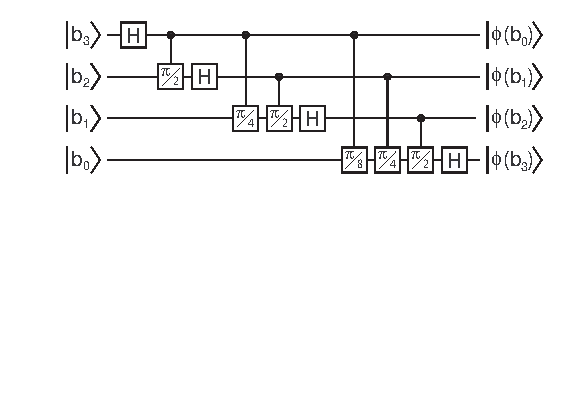
\includegraphics[width=3in]{figures/serial_qft.pdf}
\caption{The serial QFT circuit \cite{Fowler2004}.}
\label{fig:qft-serial}
\end{center}
\end{figure}

%\begin{equation}
%\label{eqn:qft-quad}
%\end{equation}

The depth and size of operations are calculated as
$\sum_{\ell=1}^n n-\ell-1 = O(n^2)$.
Also note that no ancillary qubits are needed, and the QFT is computed
in-place. Therefore the circuit width is $n$, and the circuit space is
$O(n^3)$ with an error probability of $0$ since this is an exact circuit.

%%%%%%%%%%%%%%%%%%%%%%%%%%%%%%%%%%%%%%%%%%%%%%%%%%%%%%%%%%%%%%%%%%%%%%%%%%%%%%
\subsection{QFT in $O(n\log n)$ Depth}
\label{subsec:qft-loglin}

Almost immediately after Shor's original paper, Coppersmith noted that we
could cut off the rotations $R_k$ after some maximum $k_0 = O(\log(n/\epsilon))$
and therefore decrease
our circuit size and depth to $O(n\log(n/\epsilon))$ for a given
error $\epsilon$ \cite{Coppersmith1994}. We will call this the AQFT,
for \emph{approximate QFT}. For circuits of size polynomial
in $n$, it suffices to set $\epsilon = 1/poly(n)$, and therefore our
circuit size and depth is $O(n\log(n))$. The circuit width remains the same
as before, so the circuit space is now $O(n^2\log(n))$ for
error probability $1/poly(n)$.

%%%%%%%%%%
% FIGURE %
%%%%%%%%%%
%\begin{figure}
%\label{fig:qft-approx}
%\caption{Circuit for the approximate QFT}
%\end{figure}

%%%%%%%%%%%%%%%%%%%%%%%%%%%%%%%%%%%%%%%%%%%%%%%%%%%%%%%%%%%%%%%%%%%%%%%%%%%%%%
\subsection{QFT in $O(n)$ Depth}
\label{subsec:qft-linear}

It was noted by Moore and Nilsson \cite{Moore1998} and widely attributed
to folklore that the QFT would be further parallelized by swapping qubits
so that $R_k$ rotations that operated on disjoint qubits could be executed
in the same timestep. Incidentally, this also makes the QFT implementable
on a nearest-neighbor architecture, which was discovered by Kutin, Devitt,
and Hollenberg \cite{Fowler2004} to have a pleasing triangular shape
as shown in Figure \ref{fig:qft-parallel}. This fact was later
used in the 1D NTC
architecture of Kutin \cite{Kutin2006}.

%%%%%%%%%%
% FIGURE %
%%%%%%%%%%
\begin{figure}
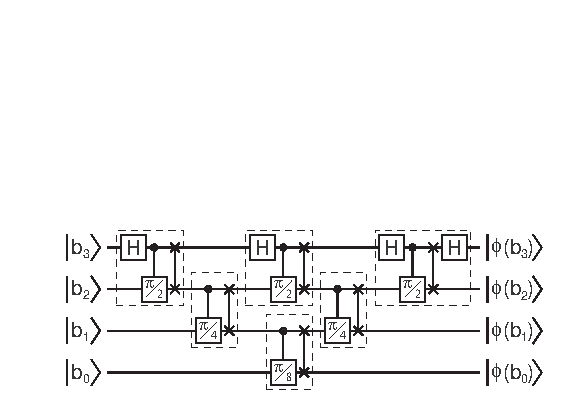
\includegraphics[width=3in]{figures/parallel_qft.pdf}
\caption{The parallel 1D NTC QFT circuit \cite{Fowler2004}.}
\label{fig:qft-parallel}
\end{figure}

This reduces the depth to $O(n)$, while the size and width remain the same
as before. Therefore, the circuit space is now $O(n^2)$, an improvement over
the AQFT in the previous section but with an error probability of $0$ since
this is an exact circuit.

%%%%%%%%%%%%%%%%%%%%%%%%%%%%%%%%%%%%%%%%%%%%%%%%%%%%%%%%%%%%%%%%%%%%%%%%%%%%%%
\subsection{QFT in Depth $O(\log n)$}
\label{subsec:qft-log}

To further exploit the fact that operations on disjoint qubits can be done
in parallel, Cleve and Watrous discovered that one could fanout the control
qubit of every $R_k$ rotation. This uses the copying technique of
Section \ref{sec:parallel}, which uses a logarithmic-depth \emph{copy network}
of
CNOT gates to create $\ell-1$ entangled copies of a source qubit
$\ket{j_\ell}$. Now every rotation controlled on $\ket{j_\ell}$ can be done
in parallel, as shown in Figure \ref{fig:qft-cw}. We can combine
this to use the
result of the approximate QFT to cut off rotations after $\log(n/\epsilon)$
bits.

\begin{figure}[!ht]
\rule{1cm}{0cm}
\setlength{\unitlength}{965sp}%
%
\begingroup\makeatletter\ifx\SetFigFont\undefined
% extract first six characters in \fmtname
\def\x#1#2#3#4#5#6#7\relax{\def\x{#1#2#3#4#5#6}}%
\expandafter\x\fmtname xxxxxx\relax \def\y{splain}%
\ifx\x\y   % LaTeX or SliTeX?
\gdef\SetFigFont#1#2#3{%
  \ifnum #1<17\tiny\else \ifnum #1<20\small\else
  \ifnum #1<24\normalsize\else \ifnum #1<29\large\else
  \ifnum #1<34\Large\else \ifnum #1<41\LARGE\else
     \huge\fi\fi\fi\fi\fi\fi
  \csname #3\endcsname}%
\else
\gdef\SetFigFont#1#2#3{\begingroup
  \count@#1\relax \ifnum 25<\count@\count@25\fi
  \def\x{\endgroup\@setsize\SetFigFont{#2pt}}%
  \expandafter\x
    \csname \romannumeral\the\count@ pt\expandafter\endcsname
    \csname @\romannumeral\the\count@ pt\endcsname
  \csname #3\endcsname}%
\fi
\fi\endgroup
\begin{picture}(8910,5495)(376,-6744)
\thinlines
\put(4801,-3061){\circle*{150}}
\put(4801,-3661){\circle*{150}}
\put(4801,-1561){\circle*{150}}
\put(4801,-2461){\circle*{150}}
\put(4801,-2161){\circle{150}}
\put(4801,-2761){\circle{150}}
\put(4801,-3361){\circle{150}}
\put(4801,-3961){\circle{150}}
\put(4801,-1561){\line( 0,-1){675}}
\put(4801,-2461){\line( 0,-1){375}}
\put(4801,-3061){\line( 0,-1){375}}
\put(4801,-3661){\line( 0,-1){375}}
\put(4201,-1561){\circle*{150}}
\put(4201,-3061){\circle*{150}}
\put(4201,-3661){\circle{150}}
\put(4201,-2461){\circle{150}}
\put(4201,-1561){\line( 0,-1){975}}
\put(4201,-3061){\line( 0,-1){675}}
\put(3601,-1561){\circle*{150}}
\put(3601,-3061){\circle{150}}
\put(3601,-1561){\line( 0,-1){1575}}
\put(7201,-3061){\circle*{150}}
\put(7201,-3661){\circle*{150}}
\put(7201,-1561){\circle*{150}}
\put(7201,-2461){\circle*{150}}
\put(7201,-2161){\circle{150}}
\put(7201,-2761){\circle{150}}
\put(7201,-3361){\circle{150}}
\put(7201,-3961){\circle{150}}
\put(7201,-1561){\line( 0,-1){675}}
\put(7201,-2461){\line( 0,-1){375}}
\put(7201,-3061){\line( 0,-1){375}}
\put(7201,-3661){\line( 0,-1){375}}
\put(7801,-1561){\circle*{150}}
\put(7801,-3061){\circle*{150}}
\put(7801,-3661){\circle{150}}
\put(7801,-2461){\circle{150}}
\put(7801,-1561){\line( 0,-1){975}}
\put(7801,-3061){\line( 0,-1){675}}
\put(8401,-1561){\circle*{150}}
\put(8401,-3061){\circle{150}}
\put(8401,-1561){\line( 0,-1){1575}}
\put(5401,-4561){\circle*{150}}
\put(5551,-4861){\circle*{150}}
\put(5701,-5161){\circle*{150}}
\put(5851,-5461){\circle*{150}}
\put(6001,-5761){\circle*{150}}
\put(6151,-6061){\circle*{150}}
\put(6301,-6361){\circle*{150}}
\put(6451,-6661){\circle*{150}}
\put(5401,-1561){\circle*{150}}
\put(5551,-2161){\circle*{150}}
\put(5701,-2461){\circle*{150}}
\put(5851,-2761){\circle*{150}}
\put(6001,-3061){\circle*{150}}
\put(6151,-3361){\circle*{150}}
\put(6301,-3661){\circle*{150}}
\put(6451,-3961){\circle*{150}}
\put(2401,-1861){\framebox(600,600){\large H}}
\put(1801,-1561){\line( 1, 0){600}}
\put(5401,-1561){\line( 0,-1){3000}}
\put(5551,-2161){\line( 0,-1){2700}}
\put(5701,-2461){\line( 0,-1){2700}}
\put(5851,-2761){\line( 0,-1){2700}}
\put(6001,-3061){\line( 0,-1){2700}}
\put(6151,-3361){\line( 0,-1){2700}}
\put(6301,-3661){\line( 0,-1){2700}}
\put(6451,-3961){\line( 0,-1){2700}}
\put(3001,-1561){\line( 1, 0){6000}}
\put(1801,-2161){\line( 1, 0){7200}}
\put(1801,-2461){\line( 1, 0){7200}}
\put(1801,-2761){\line( 1, 0){7200}}
\put(1801,-3061){\line( 1, 0){7200}}
\put(1801,-3361){\line( 1, 0){7200}}
\put(1801,-3661){\line( 1, 0){7200}}
\put(1801,-3961){\line( 1, 0){7200}}
\put(1801,-4561){\line( 1, 0){7200}}
\put(1801,-4861){\line( 1, 0){7200}}
\put(1801,-5161){\line( 1, 0){7200}}
\put(1801,-5461){\line( 1, 0){7200}}
\put(1801,-5761){\line( 1, 0){7200}}
\put(1801,-6061){\line( 1, 0){7200}}
\put(1801,-6361){\line( 1, 0){7200}}
\put(1801,-6661){\line( 1, 0){7200}}
\put(9500,-1681){\makebox(0,0)[lb]{$\ket{\mu_{0.x_j\cdots x_0}}$}}
\put(9500,-3166){\makebox(0,0)[lb]{$\ket{0^{j}}$}}
\put(9500,-4700){\makebox(0,0)[lb]{$\ket{x_j}$}}
\put(800,-4700){\makebox(0,0)[lb]{$\ket{x_j}$}}
\put(9600,-5700){\makebox(0,0)[lb]{$\vdots$}}
\put(900,-5700){\makebox(0,0)[lb]{$\vdots$}}
\put(800,-6800){\makebox(0,0)[lb]{$\ket{x_0}$}}
\put(9500,-6800){\makebox(0,0)[lb]{$\ket{x_0}$}}
\put(800,-3166){\makebox(0,0)[lb]{$\ket{0^{j}}$}}
\put(800,-1681){\makebox(0,0)[lb]{$\ket{0}$}}
\end{picture}\vspace{2mm}
\caption{QFT circuit in $O(\log n)$ depth due to Cleve and Watrous \cite{Cleve2000}.}
\label{fig:qft-cw}
\end{figure}

Furthermore, each copy network for all $n$ bits $\ket{j_\ell}$ can be done
in parallel.
Therefore, the circuit's depth is now only limited by the copy networks
and is now $O(\log n)$. The size remains unchanged asymptotically, but now
the circuit width is $O(n^2)$ to include the ancillae for the copy networks.
The circuit space is therefore $O(n^3\log\log(n/\epsilon)$. The size and
error probability is
the same as the AQFT.

%%%%%%%%%%%%%%%%%%%%%%%%%%%%%%%%%%%%%%%%%%%%%%%%%%%%%%%%%%%%%%%%%%%%%%%%%%%%%%
\subsection{QFT Summary}

Table \ref{tab:qft-summary} summarizes the circuit size, depth, width, space, and
error probability for the QFT implementations discussed in this section.
For the approximate circuits, we set $\epsilon = 1/O(n^2)$,
since this is the per-gate error we would need to get a constant
error probability for a QFT on $n$ qubits.

\begin{figure*}
\begin{center}
\begin{tabular}{|c|c|c|c|c|c|}
\hline
\textbf{Author} & \textbf{Depth} & \textbf{Size} & \textbf{Width} & \textbf{Space} & \textbf{Error}\\
\hline
Shor & $O(n^2)$ & $O(n^2)$ & $O(n)$ & $O(n^3)$ & 0\\
Coppersmith & $O(n\log n)$ & $O(n\log n)$ & $O(n)$ & $O(n^2\log n)$ & $1/O(n^2)$ \\
Folklore & $O(n)$ & $O(n^2)$ & $O(n)$ & $O(n^2)$ & 0\\
Cleve-Watrous & $O(\log n)$ & $O(n^2)$ & $O(n^2)$ & $O(n^2 \log n)$ & 0\\
Cleve-Watrous & $O(\log \log n)$ & $O(n \log n)$ & $O(n^2)$ & $O(n^2 \log\log n)$ & $1/O(n^2)$\\
Browne-Kasheffi-Perdrix & $O(1)$ & $O(n^2)$ & $O(n^2)$ & $O(n^2)$ & 0\\
\hline
\end{tabular}
\caption{Summary of circuit resources for different QFT implementations.}
\label{tab:qft-summary}
\end{center}
\end{figure*}

The result of Browne et al. \cite{Browne2009} replaces the copy network
of Cleve and Watrous with a constant-depth unbounded fan-out.
BKP can also be used to implement an
AQFT with improved circuit space, but there is no further depth improvement
possible. By introducing circuit space, we hope to provide another parameter
for continuing to improve QFT circuits in the future that will affect
practical implementations.
